\documentclass[10pt]{article}

\usepackage{fixme}
\fxsetup{ status=draft, layout=inline}
\usepackage[pdftex]{graphicx}

\ExecuteOptions{letterpaper,10pt,twocolumn,oneside,final,journal}

\begin{document}
The \fxnote{a word for ``more and more popular''} social media websites 
collect a huge amount of latent visual information for environmental and ecology monitoring.
In this work, we propose to reconstruct satellite maps of ecology status 
across North America continent 
through 12 million publicly available geo-temporal tagged images.
We select snowfall and greenary vegetation coverage as important ecology phenomena with satellite 
maps available to compare with, and straight forward \fxnote{I just want to say easy.} to identify by human. 
First we examine the existance of snow and greenery respectively on all the images and 
aggregate this result according to the geo and 
temporal attributes to make continental scale prediction over each time period. 
Then we compare our results with satellite maps for each phenomenon and find that we fill the blanket 
when satellites failed to get any data at very cloudy area or when satellite data is too 
coarse to small changes \fxnote{like vegetation case, satellite data miss data at almost all of 
the transition period}. In this case, our results are very helpful for ecologists especially when 
the data during changing or transition period is all they need without a better way to find. \fxnote{is this clear?}
We also conduct experiments with fixed time or location and find our result 
as a promising complementary of satellite maps. Moreover, we also compare the performance based on visual evidence and textual mining. 
It turns out tags can describe snowfall very well but due to \fxnote{misleading of words describing 
vegetation}, it works less satisfactory on vegetation coverage estimation.

\section{Introduction}

Monitoring the meteorology and vegetation phenomenon is the cornerstone and challenge of ecology and biology research. Expensive satellite images give large scale data but struggle with cloud cover, 
atmospheric conditions and fine-grained localization such as flower species distribution, human interaction with nature,
% and direct targeting of them, 
% \cite{China tests anti-satellite weapon, unnerving U.S., Pentagon is confident missile hit satellite tank}
% need new or more deficiency of satellites
while citizen science provides high quality data but is also costly and is very difficult to practice over large scale areas.
The enormous popularity of photo-sharing website collects images in large spatial scale, from under clouds and in close focus (compare to aerial surveillance), 
moreover, they are freely accessible to the public.
The more than 300 million images uploaded to social media every day
\cite{https://zephoria.com/top-15-valuable-facebook-statistics/}
 potentially contain not only human activities, but also outdoor ecology and biology information intentionally and incidentally as shown in Figure \ref{fig:flickrexp}.
% !! extend

The idea of reproducing satellite maps has become more and more interesting to scientists applying textual mining on \fxnote{cite{stock, ecology, election, tourists}}, 
and recently to computer vision researches directly deriving \fxnote{cite{temperature, cloud, mountain peak}} information from visual content.
In this paper, we test the feasibility of leveraging these noisy and biased images as a new approach to observe nature. We study 2 particular phenomena, snowfall and vegetation coverage as they are fundamental topic in ecology and biology study, have relatively distinct appearance to recognize, have a good chance to appear in social media, and also have satellite maps available to serve as ground truth. Our approach is illustrated in Figure \ref{fig:overview}. 
% new source of monitoring ecology information
First, we collect a large hand-labeled data set of the existence or absence of ecology phenomena. 
Then, we train a classifier for each phenomenon by combining its most discriminative visual features and by using deep learning features. 
Finally, we collect 12 million images from entire North America over 2 years, make prediction on geo and temporal scale by aggregating this visual evidence.

This paper is built on our earlier work \fxnote{cite{www}} analyzing ecology phenomenon from image tags only. We apply a new approach understanding visual content of images, and run experiments on the exact same data set to study how vision techniques could help in social media data mining compared to using textual data alone. Also, to our best knowledge, among all the research works performing social sensing with image data, this is the first one providing continental scale quantitative performance evaluation.


\begin{figure*}[h]
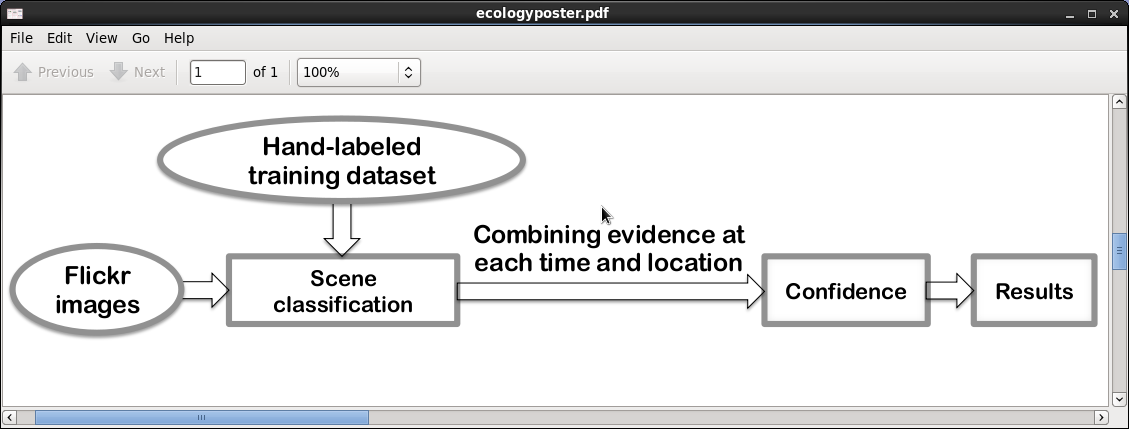
\includegraphics[scale=.3]{figure/overview.png}
\caption{Overview of our approach to apply image classifiers on large scale images and make prediction by aggregating these visual evidence. \fxnote{first classifier, then prediction}}
\label{fig:overview}
\end{figure*}


\begin{figure*}[th]
{\small{
\begin{center}
\begin{tabular}{@{}c@{\,\,\,}c@{\,\,\,}c@{\,\,\,}c@{\,\,\,}}
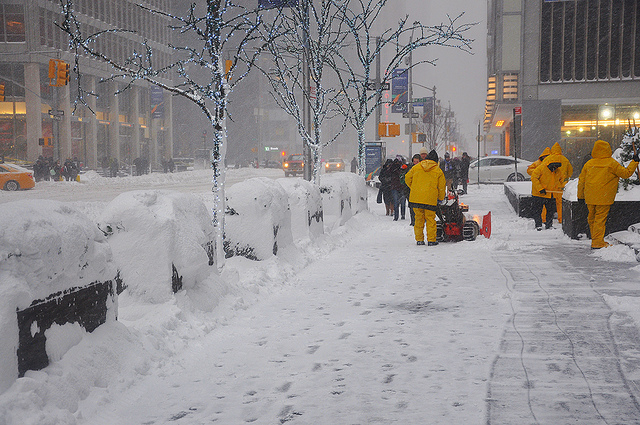
\includegraphics[width=0.19\textwidth, height=0.7in]{image/citysnow.jpg} &
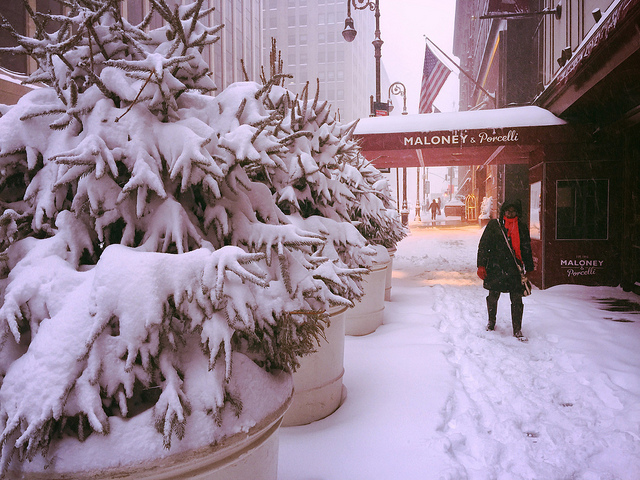
\includegraphics[width=0.19\textwidth, height=0.7in]{image/citysnow2.jpg} &
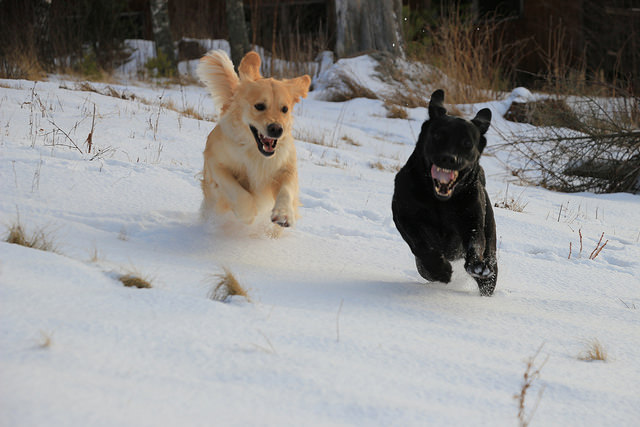
\includegraphics[width=0.19\textwidth, height=0.7in]{image/dogsnow.jpg} &
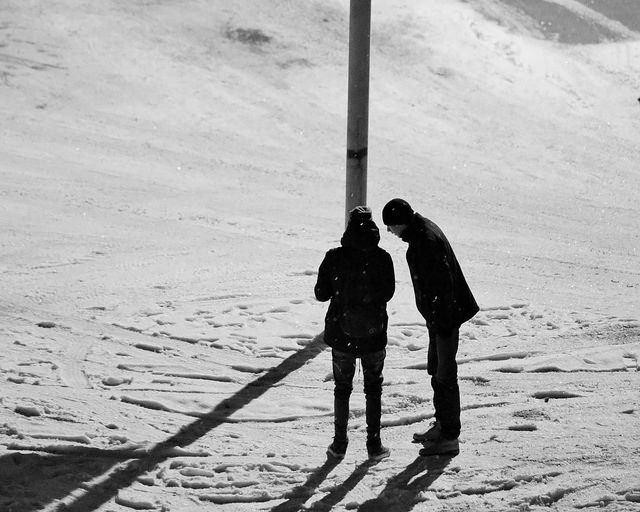
\includegraphics[width=0.19\textwidth, height=0.7in]{image/humansnow.jpg} \\
%\multicolumn{5}{c}{(a) Random positive images in vegetation dataset} \\ 
\\[-6pt]
\hline
\\[-6pt]
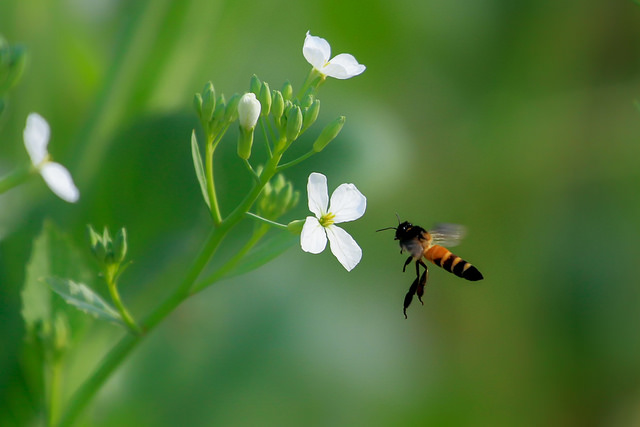
\includegraphics[width=0.19\textwidth, height=0.7in]{image/intentiongreen.jpg} &
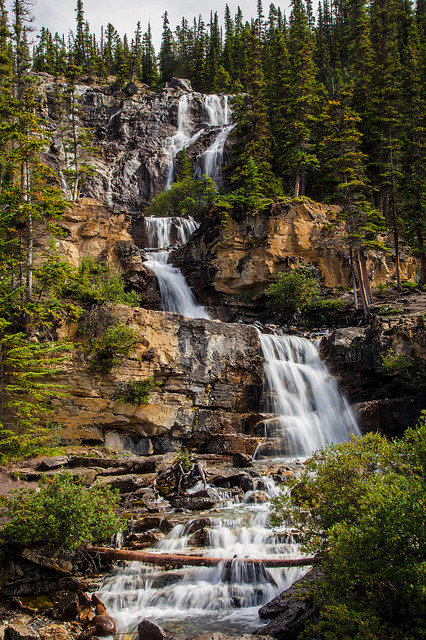
\includegraphics[width=0.19\textwidth, height=0.7in]{image/waterfallgreen.jpg} &
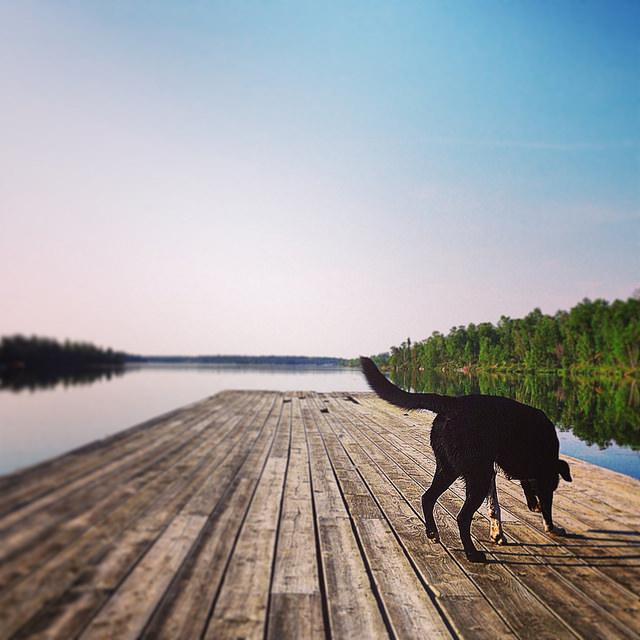
\includegraphics[width=0.19\textwidth, height=0.7in]{image/dogtree.jpg} &
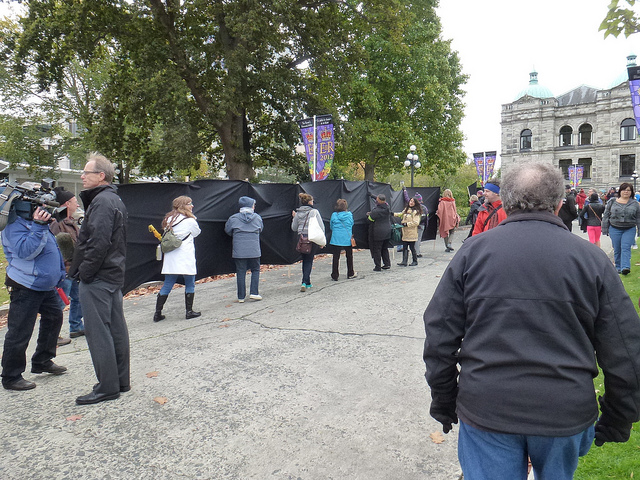
\includegraphics[width=0.19\textwidth, height=0.7in]{image/humantree.jpg} \\
%\multicolumn{5}{c}{(b) Random negative images in vegetation dataset} \\
\end{tabular}
\end{center}
}}
\caption{Flickr image examples capture snow and greenery evidence on purpose and as background.}
\label{fig:flickrexp}
\end{figure*}

%\section{Related work}
In last few years, crowd-sourcing data from social media 
as a large scale and free to public data source
has \fxnote{received lots of attention from; or (become more and more popular to)} 
researchers working on 
\fxnote{cite{old draft text mining, google doc, social event paper, 1 word for each paper, social 
before natural}}. \fxnote{talk a lot about motivation of scientific report paper}.
In \fxnote{cite{www}}, Zhang \etal estimates geo-temporal snowfall and vegetation coverage 
based on Flickr image tags.
\fxnote{accuracy of geo-temporal problem, and now it's getting better.}

Since metadata of photos provides such a huge potential in social and environmental study, it's 
natural to see a lot of works start analyzing image contents. Webcam providing dense temporal images 
is a good source to monitor the nature. A series of works \fxnote{cite{webcam papers}} 
describes outdoor scene \fxnote{cite{transattri}}, estimates \fxnote{cite{temp}} through sequences 
of webcam images. 
To evaluate the study of temperature and cloud, snowfall amount \fxnote{cite{snow on mountain peak}},
 researchers can easily compare their results with satellite data. Unfortunatelly, 
the evaluation in these works are either not on continental scale or just via quality visualization.
Social activity study on the other hand, is way more complex to evaluate the performance.

Flickr and Panaramio \fxnote{check spell} as very popular photo-sharing websites , 
``unintentionally'' \fxnote{check spell} supports researchers studies urban perception and 
\fxnote{ cite{celebrity auto tag paper} and give a term like social identity?...} and \fxnote{cite{
city attributes paper} and explain this is more important to people}. \fxnote{cite{look beyond} using 
Google Street view}.

The fact \fxnote{foundamental loop hole} that webcam can only be placed far away from people 
 makes it almost impossible to monitor people`s activity, even not the surrounding area close to
residencial or \fxnote{crowd? I mean groups of people like downtown, not ski activity but like people 
going to work and back everyday also a good topic to use temporal dense images but webcam isn't good 
at this.} Social media, on the other hand, provides a larger freedom on location distribution. 
In fact, as a complementory, almost all the photos shared online are from locations people usually go to. 
\fxnote{how helpful is this to study more areas close to urban planning, market sharing, everyday living,
anything related to people}

Our work take the advantage of studying ecology phenomena with \fxnote{easy to get, more reliable
 ground truth} and use social media data to \fxnote{monitor? insight?} these information from \fxnote{
locations more related to people}. We provide continental scale quatetive evaluation and introduce our
 method to tackle the problem of noisy and biased data, in order to support extended studies about 
more areas. \fxnote{change this sentence..}




\end{document}